\documentclass[12pt, a4paper]{article}

% ── Packages ──────────────────────────────────────────────────────────────────
\usepackage[a4paper, margin=2.5cm]{geometry}
\usepackage{graphicx}
\usepackage{float}
\usepackage{amsmath}
\usepackage{amssymb}
\usepackage{xcolor}
\usepackage{mdframed}
\usepackage{parskip}
\usepackage{enumitem}
\usepackage{titlesec}
\usepackage{booktabs}
\usepackage{hyperref}
\usepackage[T1]{fontenc}

% ── Graphics path ─────────────────────────────────────────────────────────────
\graphicspath{{figures/}}

% ── Colours ───────────────────────────────────────────────────────────────────
\definecolor{keyblue}{RGB}{30, 80, 160}
\definecolor{keybluebg}{RGB}{220, 235, 255}
\definecolor{noteorange}{RGB}{200, 100, 0}
\definecolor{noteorangebg}{RGB}{255, 240, 215}
\definecolor{warnred}{RGB}{180, 30, 30}
\definecolor{warnredbg}{RGB}{255, 220, 220}
\definecolor{defgreen}{RGB}{20, 110, 50}
\definecolor{defgreenbg}{RGB}{215, 245, 225}
\definecolor{headernavy}{RGB}{25, 35, 90}

% ── Box environments ──────────────────────────────────────────────────────────
\newmdenv[linecolor=keyblue,backgroundcolor=keybluebg,linewidth=1.5pt,
  leftline=true,rightline=false,topline=false,bottomline=false,
  innerleftmargin=10pt,innerrightmargin=8pt,
  innertopmargin=6pt,innerbottommargin=6pt,
  skipabove=8pt,skipbelow=8pt]{keybox}

\newmdenv[linecolor=noteorange,backgroundcolor=noteorangebg,linewidth=1.5pt,
  leftline=true,rightline=false,topline=false,bottomline=false,
  innerleftmargin=10pt,innerrightmargin=8pt,
  innertopmargin=6pt,innerbottommargin=6pt,
  skipabove=8pt,skipbelow=8pt]{notebox}

\newmdenv[linecolor=warnred,backgroundcolor=warnredbg,linewidth=1.5pt,
  leftline=true,rightline=false,topline=false,bottomline=false,
  innerleftmargin=10pt,innerrightmargin=8pt,
  innertopmargin=6pt,innerbottommargin=6pt,
  skipabove=8pt,skipbelow=8pt]{warnbox}

\newmdenv[linecolor=defgreen,backgroundcolor=defgreenbg,linewidth=1.5pt,
  leftline=true,rightline=false,topline=false,bottomline=false,
  innerleftmargin=10pt,innerrightmargin=8pt,
  innertopmargin=6pt,innerbottommargin=6pt,
  skipabove=8pt,skipbelow=8pt]{defbox}

% ── Section formatting ────────────────────────────────────────────────────────
\titleformat{\section}[block]{\large\bfseries\color{headernavy}}{}{0pt}{}
  [\vspace{2pt}\rule{\linewidth}{0.8pt}\vspace{4pt}]
\titleformat{\subsection}[block]{\normalsize\bfseries\color{keyblue}}{}{0pt}{}

% ── Document ──────────────────────────────────────────────────────────────────
\begin{document}

\begin{center}
  {\LARGE\bfseries\color{headernavy} Networks and Systems}\\[4pt]
  {\large MM11 --- Fault Detection via Hidden Markov Models}\\[2pt]
  {\normalsize Hans-Peter Schwefel \quad|\quad Electronic Systems, 8th Semester}
\end{center}

\vspace{4pt}\hrule height 1.2pt\vspace{12pt}

% ==============================================================================
\section*{Part 1 \quad Fault Detectors: Definition and Quality Metrics}
% ==============================================================================

% ------------------------------------------------------------------------------
\subsection*{1.1 \quad What is a Fault Detector?}
% ------------------------------------------------------------------------------

A \textbf{fault detector} is a function $\mathrm{fd}(t)$ that takes system
observations $o(t)$ as input (sampled in discrete time as $o(t_i)$) and
produces an output representing a conjecture about whether a fault is present.
The output can be:

\begin{itemize}[leftmargin=1.4em, itemsep=3pt]
  \item \textbf{Binary}: $\mathrm{fd}(t) = 1$ if a fault is detected, $0$ otherwise.
  \item \textbf{Probabilistic}: $\mathrm{fd}(t) \in [0, 1]$, representing an estimated
    probability of a fault being present.
\end{itemize}

The \textbf{ideal fault detector} outputs exactly $1$ whenever the fault is
present and $0$ otherwise. In practice this ideal is never achieved, and we
instead characterise detectors by their error metrics.

% ------------------------------------------------------------------------------
\subsection*{1.2 \quad Example: Detection of Node Crashes}
% ------------------------------------------------------------------------------

A common practical problem is determining whether a remote host is up or down.
Two time-out based strategies are used:

\begin{figure}[H]
  \centering
  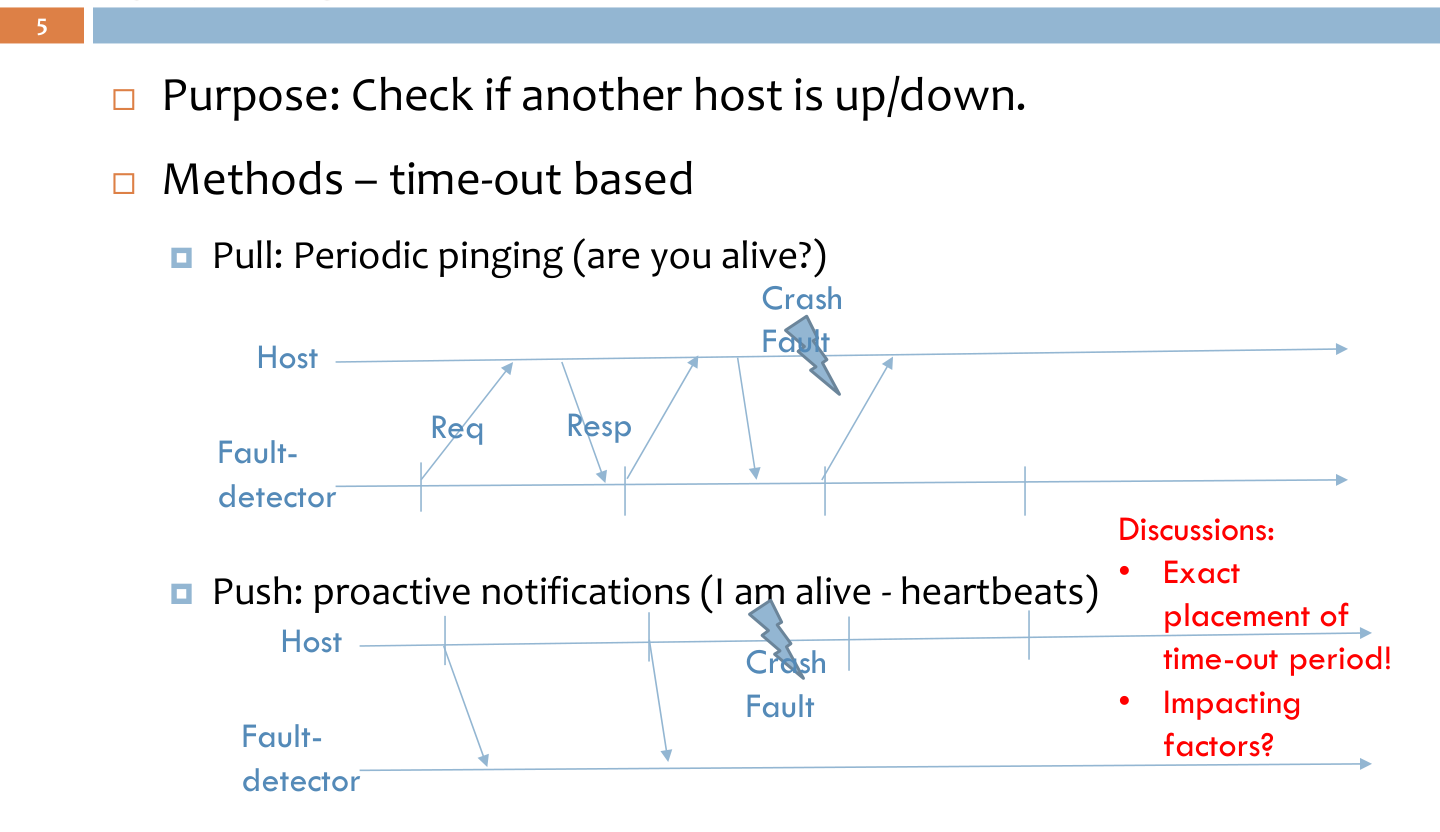
\includegraphics[width=0.85\textwidth]{fig_node_crash.png}
  \caption{Two approaches to crash detection.
    \textbf{Pull} (top): the fault detector sends periodic ping requests and
    waits for a response. If no response arrives within the time-out window, a
    fault is declared.
    \textbf{Push} (bottom): the host sends heartbeat messages proactively; the
    detector declares a fault if a heartbeat is missed.
    Key design question: where exactly should the time-out period be placed, and
    what factors (network delay, jitter, load) affect it?}
\end{figure}

\begin{notebox}
  \textbf{Design trade-off for the time-out period}

  A \emph{short} time-out reacts quickly to crashes (low reactivity time) but
  generates false alarms whenever a reply is merely delayed.
  A \emph{long} time-out avoids false alarms but slows down crash detection.
  Choosing the right value requires knowledge of the round-trip time
  distribution under normal operation.
\end{notebox}

% ------------------------------------------------------------------------------
\subsection*{1.3 \quad True/False Positives and Negatives --- The Confusion Matrix}
% ------------------------------------------------------------------------------

When evaluating any fault detector we need a way to \emph{score} its
performance. The fundamental idea is simple: at every point in time the system
is either actually faulty or not, and the detector either alarms or it does not.
Crossing these two binary facts gives four possible outcomes. The
\textbf{confusion matrix} is just a table that organises these four cases and
asks the question: \emph{how often does each case occur?}

\begin{figure}[H]
  \centering
  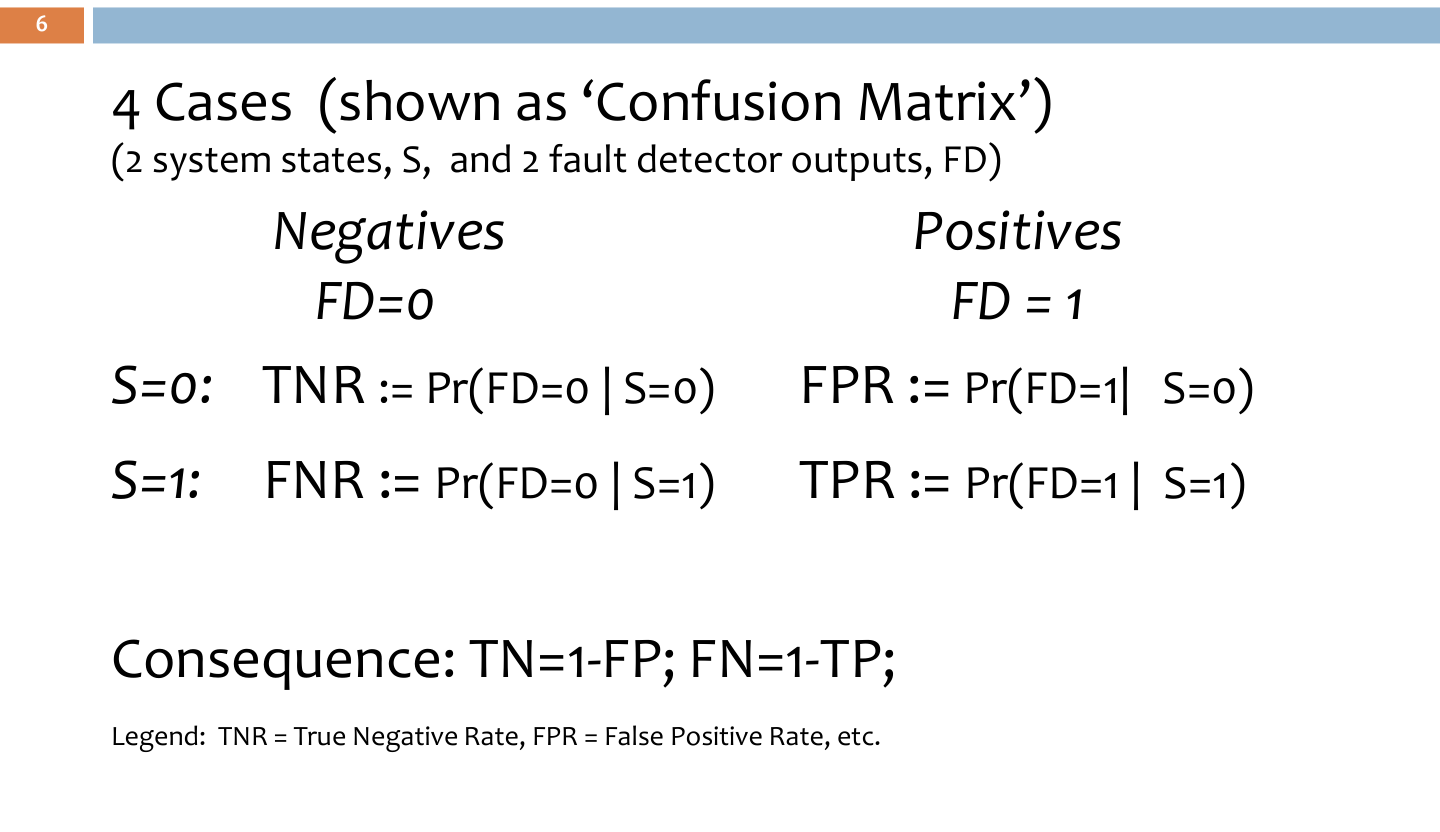
\includegraphics[width=0.75\textwidth]{fig_confusion_matrix.png}
  \caption{The four outcomes formed by crossing the true system state $S$ with
    the fault-detector output FD. Each cell is labelled TP, TN, FP, or FN
    depending on whether the detector was correct (True) or wrong (False), and
    whether it alarmed (Positive) or stayed silent (Negative).}
\end{figure}

To be precise, we work with \emph{rates} (probabilities) rather than raw
counts, because the absolute number of events depends on how long we observe
the system. With $S \in \{0,1\}$ denoting the true system state and
$\mathrm{FD} \in \{0,1\}$ the detector output, the four conditional
probabilities are:

\begin{center}
\begin{tabular}{lll}
\toprule
 & $\mathrm{FD}=0$ (silent) & $\mathrm{FD}=1$ (alarm) \\
\midrule
$S=0$ (no fault) & $\mathrm{TNR} = \Pr(\mathrm{FD}=0 \mid S=0)$ & $\mathrm{FPR} = \Pr(\mathrm{FD}=1 \mid S=0)$ \\
$S=1$ (fault)    & $\mathrm{FNR} = \Pr(\mathrm{FD}=0 \mid S=1)$ & $\mathrm{TPR} = \Pr(\mathrm{FD}=1 \mid S=1)$ \\
\bottomrule
\end{tabular}
\end{center}

Where each abbreviation stands for:
\begin{itemize}[leftmargin=1.4em, itemsep=3pt]
  \item \textbf{TNR} --- True Negative Rate: the system is healthy and the
    detector correctly stays silent. This is what we want during normal
    operation.
  \item \textbf{FPR} --- False Positive Rate: the system is healthy but the
    detector fires anyway. This is a \emph{false alarm} --- annoying and
    potentially costly because operators may react unnecessarily.
  \item \textbf{FNR} --- False Negative Rate: the system is faulty but the
    detector says nothing. This is a \emph{missed fault} --- the most dangerous
    outcome, as a real problem goes unnoticed.
  \item \textbf{TPR} --- True Positive Rate (also called \emph{sensitivity} or
    \emph{recall}): the system is faulty and the detector correctly alarms.
    This is what we want during a fault.
\end{itemize}

Because each row of the table describes all outcomes for one system state, each
row must sum to 1. This gives the key identities:
\[
  \mathrm{TNR} = 1 - \mathrm{FPR}, \qquad \mathrm{FNR} = 1 - \mathrm{TPR}.
\]
\begin{itemize}[leftmargin=1.4em, itemsep=2pt]
  \item $\mathrm{TNR}$ --- True Negative Rate (probability of silence when healthy).
  \item $\mathrm{FPR}$ --- False Positive Rate (probability of alarm when healthy).
  \item $\mathrm{FNR}$ --- False Negative Rate (probability of silence when faulty).
  \item $\mathrm{TPR}$ --- True Positive Rate (probability of alarm when faulty).
\end{itemize}

This means we only need \emph{one} number per row to describe everything.
In practice FPR and TPR are chosen as the two summary metrics because they
correspond directly to the two costs we care about: unnecessary alarms and
missed faults.

\textbf{Accuracy} summarises the overall correctness of the detector in a
single number:
\[
  \mathrm{Accuracy} = \Pr(\mathrm{FD} = S)
  = \mathrm{TPR} \cdot \Pr(S=1) + \mathrm{TNR} \cdot \Pr(S=0).
\]
\begin{itemize}[leftmargin=1.4em, itemsep=2pt]
  \item $\mathrm{Accuracy}$ --- probability that detector output matches the
    true system state at any given moment.
  \item $\mathrm{TPR}$ --- True Positive Rate (how often we alarm when faulty).
  \item $\mathrm{TNR}$ --- True Negative Rate (how often we stay silent when healthy).
  \item $\Pr(S=1)$ --- prior probability that the system is currently faulty
    (depends on how reliable the system is overall).
  \item $\Pr(S=0)$ --- prior probability that the system is currently healthy.
\end{itemize}

\begin{warnbox}
  \textbf{Accuracy can be misleading.}
  Consider a system that is faulty only $1\%$ of the time ($\Pr(S=1)=0.01$).
  A detector that \emph{never} fires achieves $99\%$ accuracy --- yet it is
  completely useless because it never detects anything.
  This is why FPR and TPR (and the ROC curve, Section~2.2) are preferred over
  accuracy alone.
\end{warnbox}

% ------------------------------------------------------------------------------
\subsection*{1.4 \quad Reactivity and the Full Metrics Picture}
% ------------------------------------------------------------------------------

\begin{figure}[H]
  \centering
  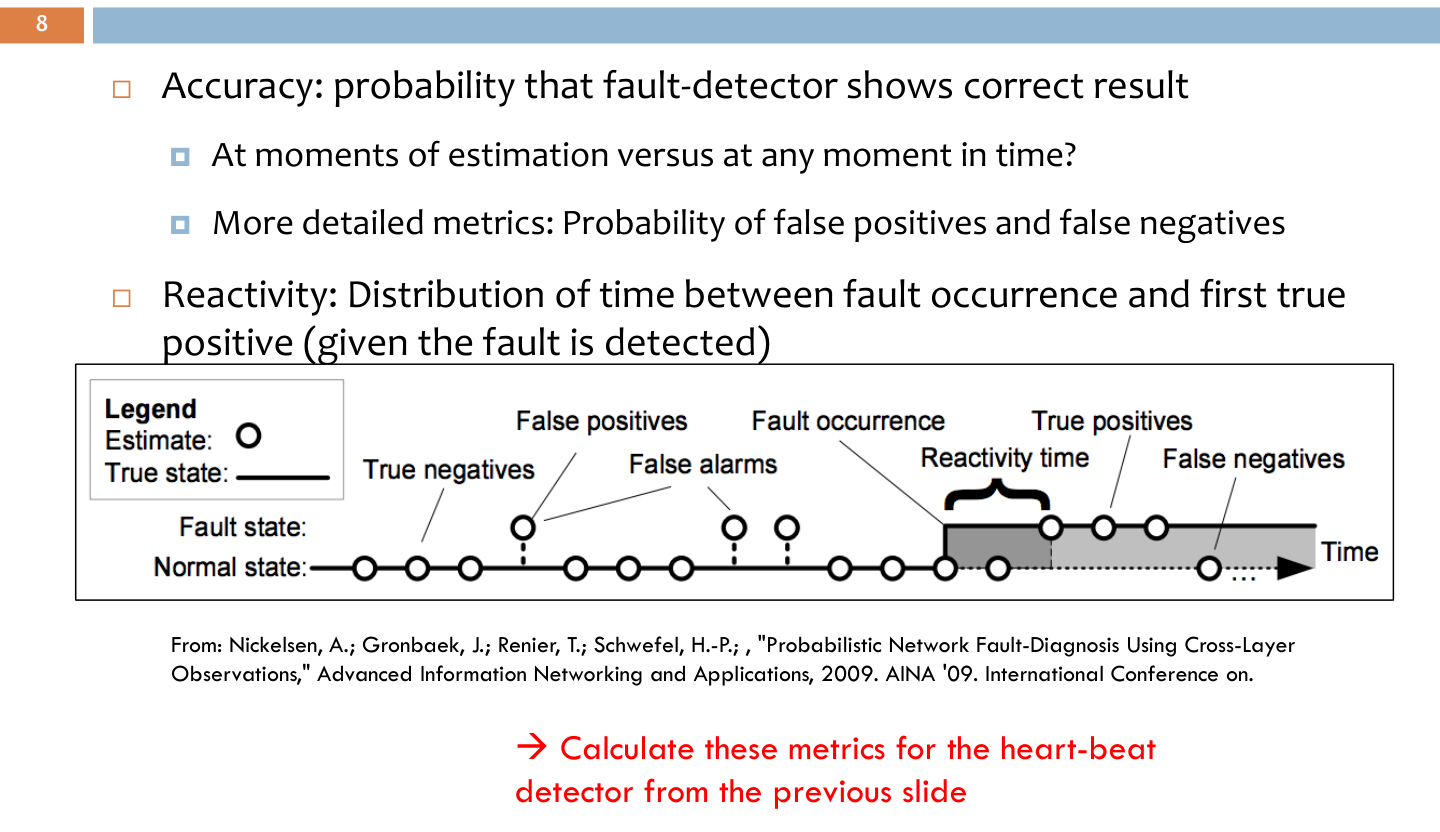
\includegraphics[width=\textwidth]{fig_metrics_timeline.png}
  \caption{A timeline showing all four outcomes over time for one fault event.
    Before the fault: the detector's silence counts as True Negatives (TN),
    while any spurious alarm counts as a False Positive (FP, also called a
    false alarm). After the fault occurs, there is a window where the detector
    has not yet reacted --- outputs here are False Negatives (FN). Once the
    detector finally fires, we enter the True Positive (TP) region.
    The width of the FN window is the \emph{reactivity time}.}
\end{figure}

\begin{defbox}
  \textbf{Reactivity} is the distribution of the time elapsed between
  fault occurrence and the \emph{first} true-positive output of the detector
  (given that the fault is eventually detected).
  It quantifies how fast the detector responds.
  A short reactivity is desirable but typically comes at the cost of more false
  positives.
\end{defbox}

In other words: FPR and FNR/TPR tell us \emph{how often} the detector is
right or wrong; reactivity tells us \emph{how quickly} it notices when something
goes wrong. A good detector needs to balance all three.

% ==============================================================================
\section*{Part 2 \quad Threshold Detectors and ROC Curves}
% ==============================================================================

% ------------------------------------------------------------------------------
\subsection*{2.1 \quad Example: Congestion Detection via RTT}
% ------------------------------------------------------------------------------

A simple but practically important fault detector uses round-trip time (RTT)
measurements to decide whether a network path is congested.
The idea is straightforward: when a network is congested, packets spend more
time queuing in routers, so the RTT grows. If the RTT exceeds some chosen
limit, we declare congestion. Formally the detection rule is:
\[
  \mathrm{FD}(t_i) = \mathbf{1}\!\left[\mathrm{RTT}_i > \theta\right],
\]
\begin{itemize}[leftmargin=1.4em, itemsep=2pt]
  \item $\mathrm{FD}(t_i)$ --- fault detector output at time step $t_i$; equals
    $1$ (congestion declared) or $0$ (no congestion).
  \item $\mathrm{RTT}_i$ --- round-trip time measured at time step $i$, in
    milliseconds.
  \item $\theta$ --- the detection \textbf{threshold}; the single tuning
    parameter of this detector.
  \item $\mathbf{1}[\cdot]$ --- indicator function; equals $1$ if the condition
    inside is true, $0$ otherwise.
\end{itemize}

The key question is: what should $\theta$ be? To answer this we need to look
at the RTT distributions under the two possible system states.

\begin{figure}[H]
  \centering
  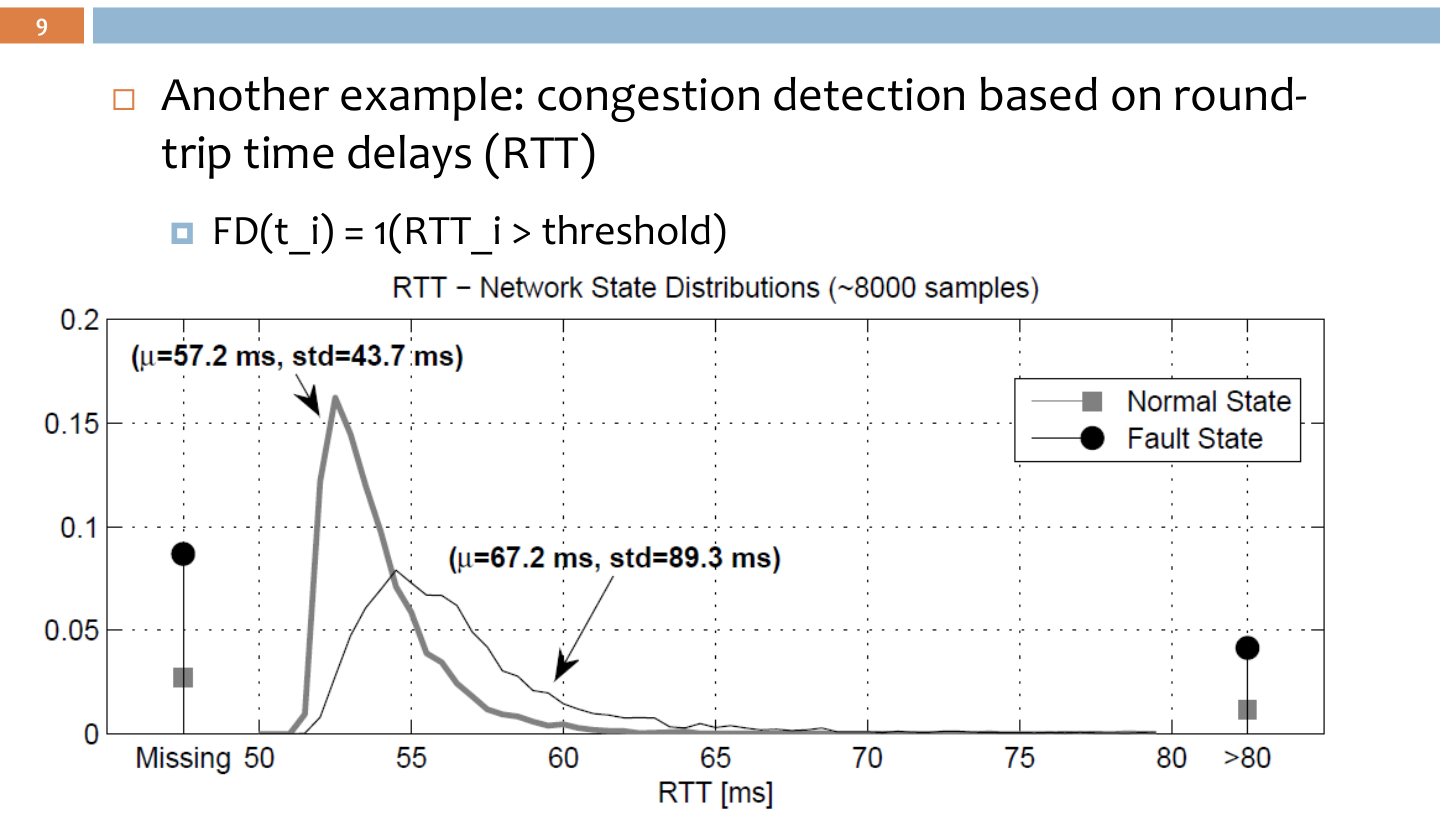
\includegraphics[width=0.85\textwidth]{fig_rtt_distributions.png}
  \caption{RTT probability distributions measured from approximately 8000
    samples, shown separately for the \textbf{normal state} (narrow peak,
    $\mu = 57.2\,\mathrm{ms}$, $\sigma = 43.7\,\mathrm{ms}$) and the
    \textbf{fault/congestion state} (much wider and heavier-tailed,
    $\mu = 67.2\,\mathrm{ms}$, $\sigma = 89.3\,\mathrm{ms}$).
    The $x$-axis is the RTT value in milliseconds; the $y$-axis is the
    probability of observing that RTT value.
    Notice that the two distributions overlap substantially in the
    50--65\,ms region, which means no single threshold can perfectly separate
    them.}
\end{figure}

The figure shows the core problem: the normal-state distribution and the
fault-state distribution are not perfectly separated --- they overlap.
Every RTT value in the overlap region is ambiguous: it could have come from
either state. No matter where we place the threshold $\theta$, we will
inevitably misclassify some samples. Moving $\theta$ to the left catches more
faults (higher TPR) but also flags more healthy samples as congested (higher
FPR). Moving $\theta$ to the right reduces false alarms (lower FPR) but
misses more real faults (lower TPR). This is the fundamental trade-off.

\begin{figure}[H]
  \centering
  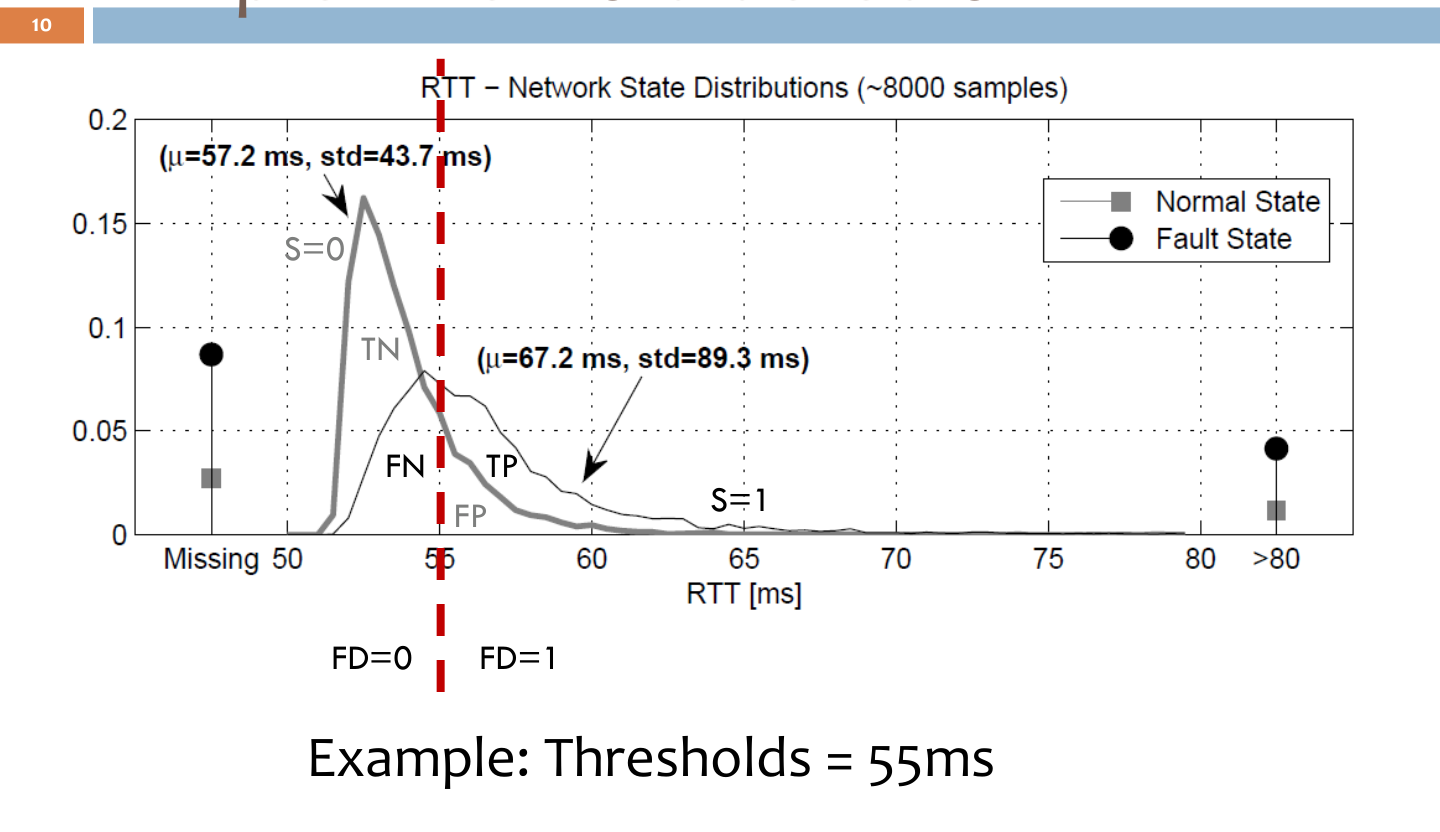
\includegraphics[width=0.85\textwidth]{fig_threshold_confusion.png}
  \caption{Visual derivation of the confusion matrix for a threshold of
    $\theta = 55\,\mathrm{ms}$ (the vertical red dashed line).
    Everything to the \textbf{left} of the line is labelled $\mathrm{FD}=0$
    (no fault declared); everything to the \textbf{right} is $\mathrm{FD}=1$
    (fault declared).
    For the $S=0$ (normal) curve: the area to the left is TN (correctly silent)
    and the area to the right is FP (false alarm).
    For the $S=1$ (fault) curve: the area to the left is FN (missed fault) and
    the area to the right is TP (correct detection).
    The relative sizes of these areas give the TNR, FPR, FNR, and TPR for this
    particular choice of $\theta$.}
\end{figure}

This figure is the geometric version of the confusion matrix. Instead of
abstract probabilities, you can literally see the four regions on the
distribution plot. Choosing $\theta = 55\,\mathrm{ms}$ already catches a
reasonable portion of the fault distribution on the right, but still leaves
some of the normal distribution on the right as false positives.

% ------------------------------------------------------------------------------
\subsection*{2.2 \quad ROC Curves}
% ------------------------------------------------------------------------------

Since there are infinitely many possible values of $\theta$, and each gives a
different (FPR, TPR) pair, we need a way to visualise the \emph{full range} of
trade-offs available. That is exactly what the \textbf{ROC curve} does: it
sweeps $\theta$ from $-\infty$ to $+\infty$ and plots the resulting (FPR, TPR)
pairs as a curve in 2D space. Each point on the curve is one detector
configuration; the curve as a whole is the performance landscape.

\begin{figure}[H]
  \centering
  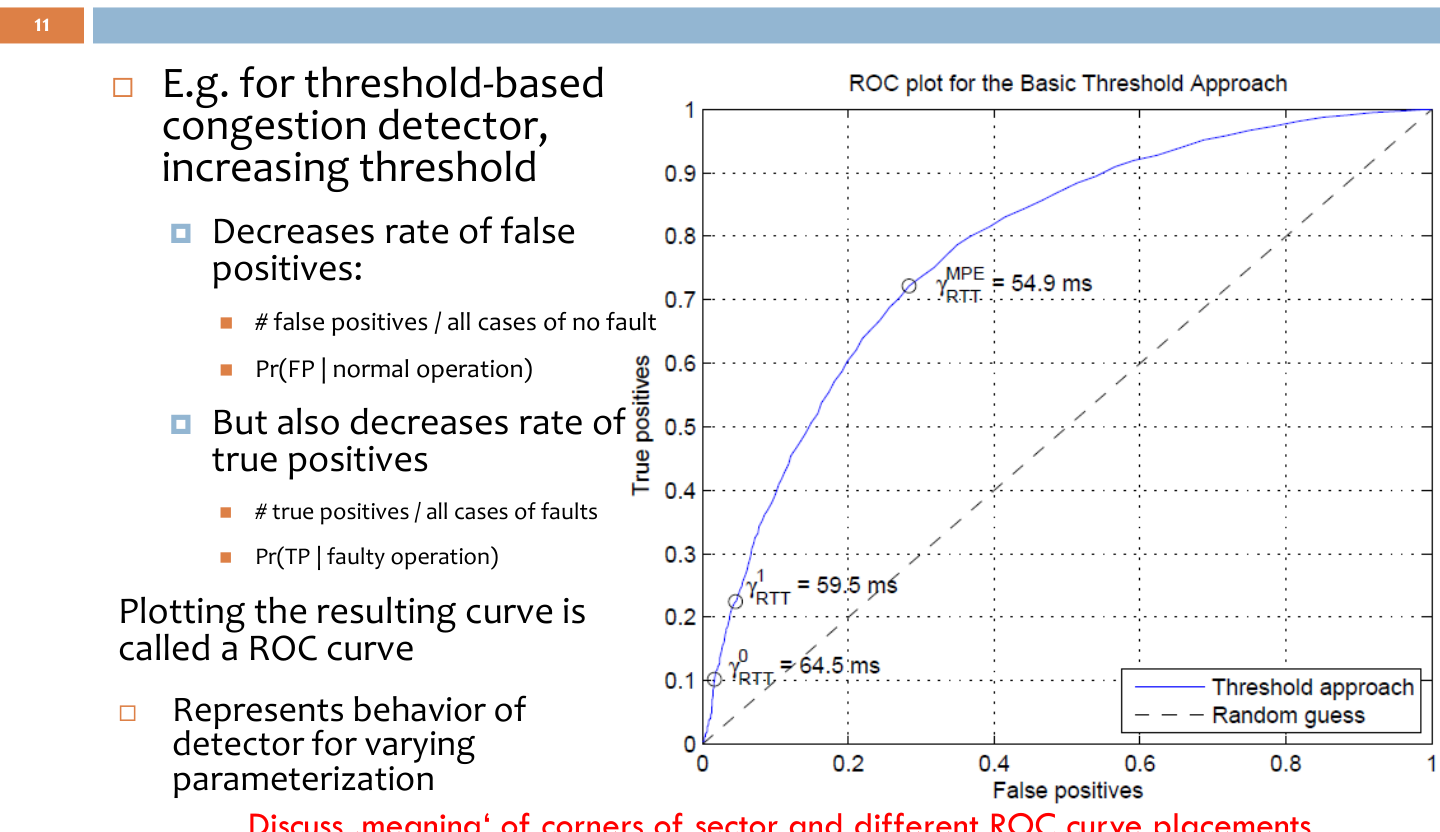
\includegraphics[width=0.85\textwidth]{fig_roc_curve.png}
  \caption{ROC (Receiver Operating Characteristic) curve for the
    threshold-based congestion detector using RTT measurements.
    The $x$-axis is the False Positive Rate (FPR) and the $y$-axis is the
    True Positive Rate (TPR).
    Each labelled point corresponds to a specific threshold value (e.g.\
    $\theta_{\mathrm{RTT}}^0 = 64.5\,\mathrm{ms}$ near the bottom-left).
    As $\theta$ decreases, the operating point moves up and to the right ---
    more faults caught, but more false alarms too.
    The dashed diagonal represents a random-guess detector (TPR $=$ FPR).}
\end{figure}

\begin{keybox}
  \textbf{Reading a ROC curve --- what each corner means}
  \begin{itemize}[leftmargin=1.2em, itemsep=3pt]
    \item \textbf{Top-left corner} $(0,\,1)$: the ideal detector. It never
      false-alarms (FPR $= 0$) and always catches faults (TPR $= 1$). Every
      real detector falls short of this.
    \item \textbf{Bottom-left corner} $(0,\,0)$: the detector that always says
      ``no fault.'' Zero false alarms, but also zero fault detections.
      This corresponds to a threshold of $+\infty$.
    \item \textbf{Top-right corner} $(1,\,1)$: the detector that always says
      ``fault.'' Catches every real fault, but also alarms on every healthy
      sample. This corresponds to a threshold of $-\infty$.
    \item \textbf{The diagonal} from $(0,0)$ to $(1,1)$: the performance of a
      completely random detector (e.g.\ flipping a coin). Any useful detector
      must lie \emph{above} the diagonal.
  \end{itemize}
  A curve that bulges strongly towards the top-left is better than one hugging
  the diagonal. The ROC curve also lets you pick the threshold that gives the
  best balance for your specific application (e.g.\ prefer low FPR for a
  safety-critical system, or high TPR if missing faults is very costly).
\end{keybox}

% ==============================================================================
\section*{Part 3 \quad Discrete-Time Markov Chains (Revision)}
% ==============================================================================

% ------------------------------------------------------------------------------
\subsection*{3.1 \quad Definition and Key Properties}
% ------------------------------------------------------------------------------

A \textbf{discrete-time Markov chain (DTMC)} is a probabilistic model for a
system that jumps between a set of states at regular time steps. It is the
building block we need before defining an HMM.

A DTMC is defined by three ingredients:
\begin{itemize}[leftmargin=1.4em, itemsep=3pt]
  \item A finite (or countable) \textbf{state space} $E = \{1, 2, \ldots, N\}$
    --- the set of all possible conditions the system can be in.
  \item \textbf{Transition probabilities} $p_{jk} = \Pr(X_{i} = k \mid X_{i-1} = j)$
    --- the probability of moving from state $j$ to state $k$ in one step.
    All $p_{jk}$ are collected in the $N \times N$ \textbf{transition matrix}
    $\mathbf{P}$, where row $j$ sums to 1.
  \item An \textbf{initial distribution} $\boldsymbol{\pi}_0$ --- a probability
    vector describing the likelihood of starting in each state.
\end{itemize}

The fundamental \textbf{Markov property} is what makes the model tractable:
the state at the next step depends \emph{only} on the current state, not on
how we got there. Formally:
\[
  \Pr(X_i = s \mid X_{i-1} = s_{i-1}, X_{i-2} = s_{i-2}, \ldots, X_0 = s_0)
  = \Pr(X_i = s \mid X_{i-1} = s_{i-1}).
\]
\begin{itemize}[leftmargin=1.4em, itemsep=2pt]
  \item $X_i$ --- the random variable representing the system state at step $i$.
  \item $s, s_{i-1}, \ldots, s_0$ --- specific values (realisations) of the
    state at each time step.
  \item The left-hand side conditions on the entire history; the right-hand side
    shows it simplifies to conditioning only on the previous step.
\end{itemize}

This ``memoryless'' property means we can propagate the state-probability
vector one step at a time using a simple matrix multiplication:
\[
  \boldsymbol{\pi}_i = \boldsymbol{\pi}_{i-1}\,\mathbf{P}.
\]
\begin{itemize}[leftmargin=1.4em, itemsep=2pt]
  \item $\boldsymbol{\pi}_i$ --- a row vector of length $N$ where entry $k$
    gives $\Pr(X_i = k)$, the probability of being in state $k$ at step $i$.
  \item $\boldsymbol{\pi}_{i-1}$ --- the same vector one step earlier.
  \item $\mathbf{P}$ --- the $N \times N$ transition matrix.
\end{itemize}

For an \textbf{ergodic} chain (one that is irreducible, meaning every state
can be reached from every other state, and aperiodic, meaning it does not get
stuck in a cycle) the distribution converges to a unique
\textbf{steady-state} $\boldsymbol{\pi}$ regardless of the starting point:
\[
  \boldsymbol{\pi} = \lim_{i \to \infty} \boldsymbol{\pi}_i,
  \qquad \text{satisfying} \qquad
  \boldsymbol{\pi} = \boldsymbol{\pi}\,\mathbf{P}.
\]
\begin{itemize}[leftmargin=1.4em, itemsep=2pt]
  \item $\boldsymbol{\pi}$ --- the steady-state (stationary) distribution; a
    row vector that is a \emph{left eigenvector} of $\mathbf{P}$ with
    eigenvalue 1.
  \item $\boldsymbol{\pi} = \boldsymbol{\pi}\,\mathbf{P}$ --- this equation
    says ``if the distribution is already $\boldsymbol{\pi}$, applying one
    more step of $\mathbf{P}$ leaves it unchanged.''
  \item In practice, $\boldsymbol{\pi}$ is found by solving this equation and
    normalising so that the entries sum to 1.
\end{itemize}

% ------------------------------------------------------------------------------
\subsection*{3.2 \quad Wireless Link Example}
% ------------------------------------------------------------------------------

As a concrete example, consider a wireless link whose quality fluctuates over
time. We model this with three states and assume time steps of one second.

\begin{figure}[H]
  \centering
  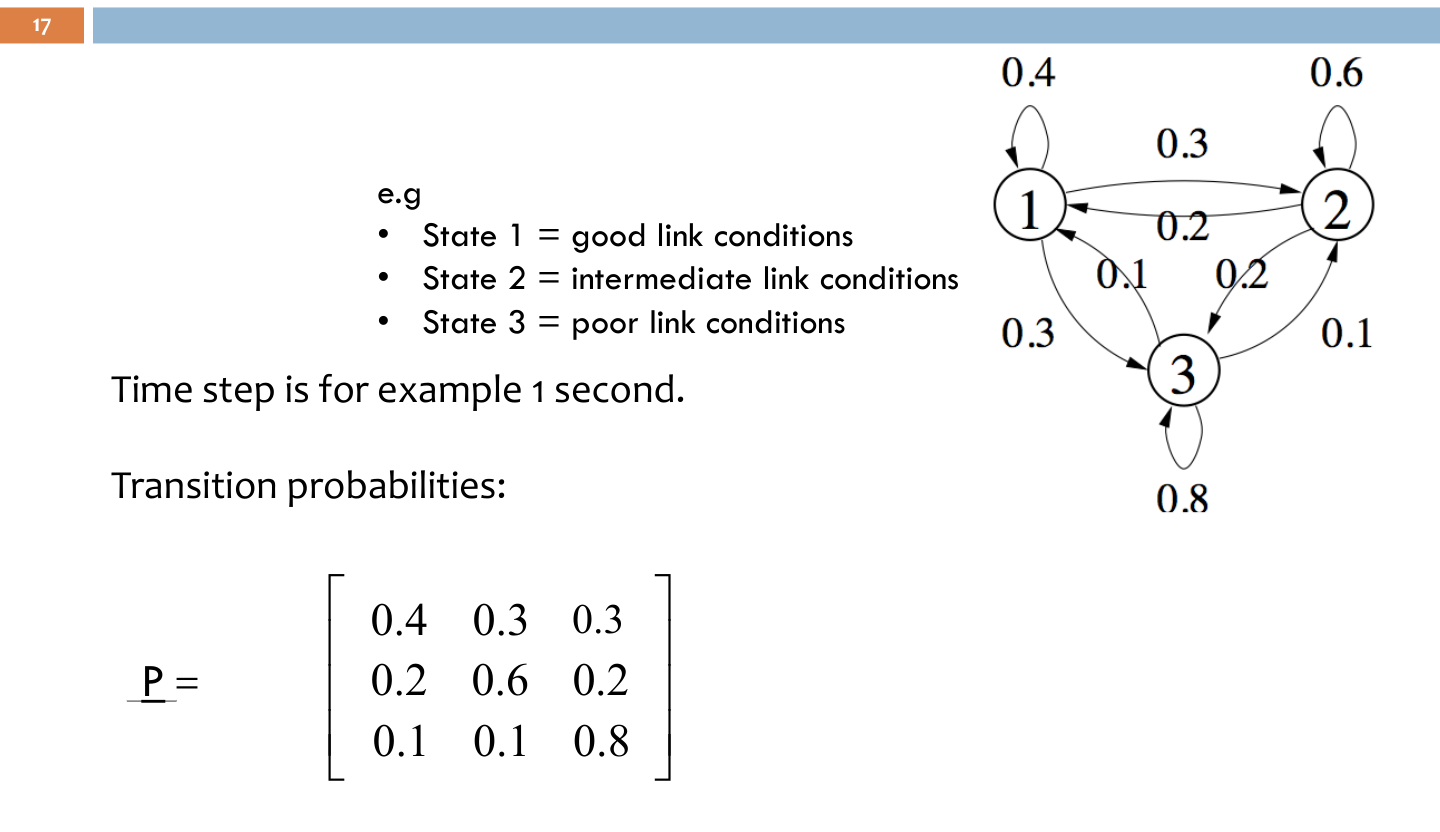
\includegraphics[width=0.85\textwidth]{fig_wireless_mc.png}
  \caption{Three-state Markov chain for wireless link quality.
    \textbf{State 1} = good link conditions,
    \textbf{State 2} = intermediate link conditions,
    \textbf{State 3} = poor link conditions.
    The directed graph shows the transition probabilities on each arrow;
    self-loops are the probabilities of staying in the same state.
    The transition matrix $\mathbf{P}$ is shown in the lower-left.
    Notice that State 3 (poor) has the largest self-loop probability
    ($p_{33} = 0.8$), meaning poor conditions tend to persist once they occur.}
\end{figure}

The matrix $\mathbf{P}$ is read row by row: row $j$ gives the probability
distribution over the next state, given that the current state is $j$.
For instance, if the link is currently in State 1 (good), there is a $0.4$
probability of staying good, $0.3$ of moving to intermediate, and $0.3$ of
deteriorating to poor.

\begin{figure}[H]
  \centering
  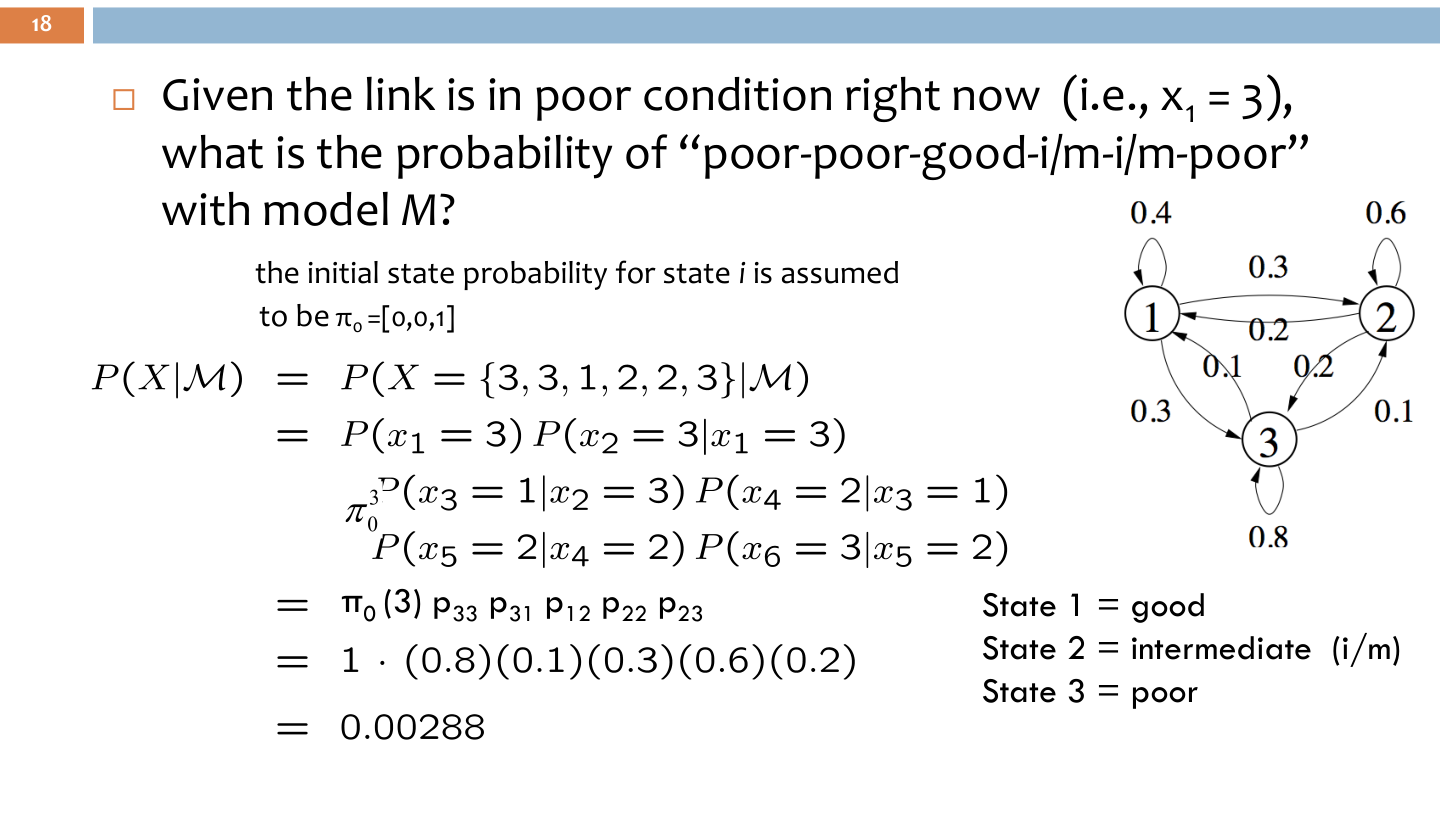
\includegraphics[width=0.90\textwidth]{fig_wireless_example2.png}
  \caption{Worked probability calculation for the specific state sequence
    $\mathbf{x} = \{3, 3, 1, 2, 2, 3\}$ (poor $\to$ poor $\to$ good
    $\to$ intermediate $\to$ intermediate $\to$ poor), starting from
    $\boldsymbol{\pi}_0 = [0,\,0,\,1]$ (certainty of starting in State 3).
    The probability is computed as a chain of transition probabilities along
    the path, yielding $0.00288$.}
\end{figure}

The calculation in the figure shows the general rule for computing the
probability of any specific state sequence $\mathbf{x} = \{x_1, x_2,
\ldots, x_T\}$:
\[
  \Pr(\mathbf{X} = \mathbf{x}) = \pi_0(x_1) \cdot p_{x_1 x_2} \cdot p_{x_2 x_3}
  \cdots p_{x_{T-1} x_T}.
\]
\begin{itemize}[leftmargin=1.4em, itemsep=2pt]
  \item $\pi_0(x_1)$ --- the initial probability of starting in state $x_1$.
    Here $\pi_0(3) = 1$ since we start in State 3 with certainty.
  \item $p_{x_t x_{t+1}}$ --- the transition probability from state $x_t$ to
    state $x_{t+1}$; read from row $x_t$, column $x_{t+1}$ of $\mathbf{P}$.
  \item The product runs over all $T-1$ consecutive state transitions in the
    sequence.
\end{itemize}

For the example sequence $\{3,3,1,2,2,3\}$:
\[
  \Pr = 1 \cdot \underbrace{0.8}_{p_{33}} \cdot \underbrace{0.1}_{p_{31}}
      \cdot \underbrace{0.3}_{p_{12}} \cdot \underbrace{0.6}_{p_{22}}
      \cdot \underbrace{0.2}_{p_{23}} = 0.00288.
\]

% ==============================================================================
\section*{Part 4 \quad Hidden Markov Models}
% ==============================================================================

% ------------------------------------------------------------------------------
\subsection*{4.1 \quad Motivation --- Why ``Hidden''?}
% ------------------------------------------------------------------------------

In the wireless link example of Part~3 we assumed we could \emph{directly
observe} the link state (good/intermediate/poor). In reality, this is almost
never the case. What a device can actually observe is the \emph{outcome of
transmissions} --- each frame either arrives correctly (C) or with an error
(E). The link state drives these outcomes but is itself invisible.

The frame-error rate (FER) depends on the hidden state:
\[
  \mathrm{FER}(\text{good}) = 10^{-5}, \qquad
  \mathrm{FER}(\text{i/m}) = 0.02, \qquad
  \mathrm{FER}(\text{poor}) = 0.2.
\]
\begin{itemize}[leftmargin=1.4em, itemsep=2pt]
  \item $\mathrm{FER}(s)$ --- frame error rate when the link is in state $s$;
    i.e.\ the probability that any given frame is received in error.
  \item The values say: in good conditions errors are extremely rare
    ($10^{-5}$), in intermediate conditions roughly 1-in-50 frames fail
    (0.02), and in poor conditions 1-in-5 fail (0.2).
\end{itemize}

Now consider what we can infer. If we observe the sequence \texttt{CCCC}
(four correct frames in a row), the link is probably in a good or intermediate
state. If we see \texttt{EEEE} (four errors in a row), it is almost certainly
in a poor state. But what about \texttt{CCCE}? The single error could be
noise in an otherwise good link, or it could be the start of a deterioration.
Deciding this rigorously --- and computing an actual probability --- is
exactly what a \textbf{Hidden Markov Model} lets us do.

The word ``hidden'' refers to the fact that the \emph{state} of the Markov
chain is not directly observed; only the \emph{emission} (the symbol produced
by that state) is observable.

% ------------------------------------------------------------------------------
\subsection*{4.2 \quad Definition of an HMM}
% ------------------------------------------------------------------------------

\begin{figure}[H]
  \centering
  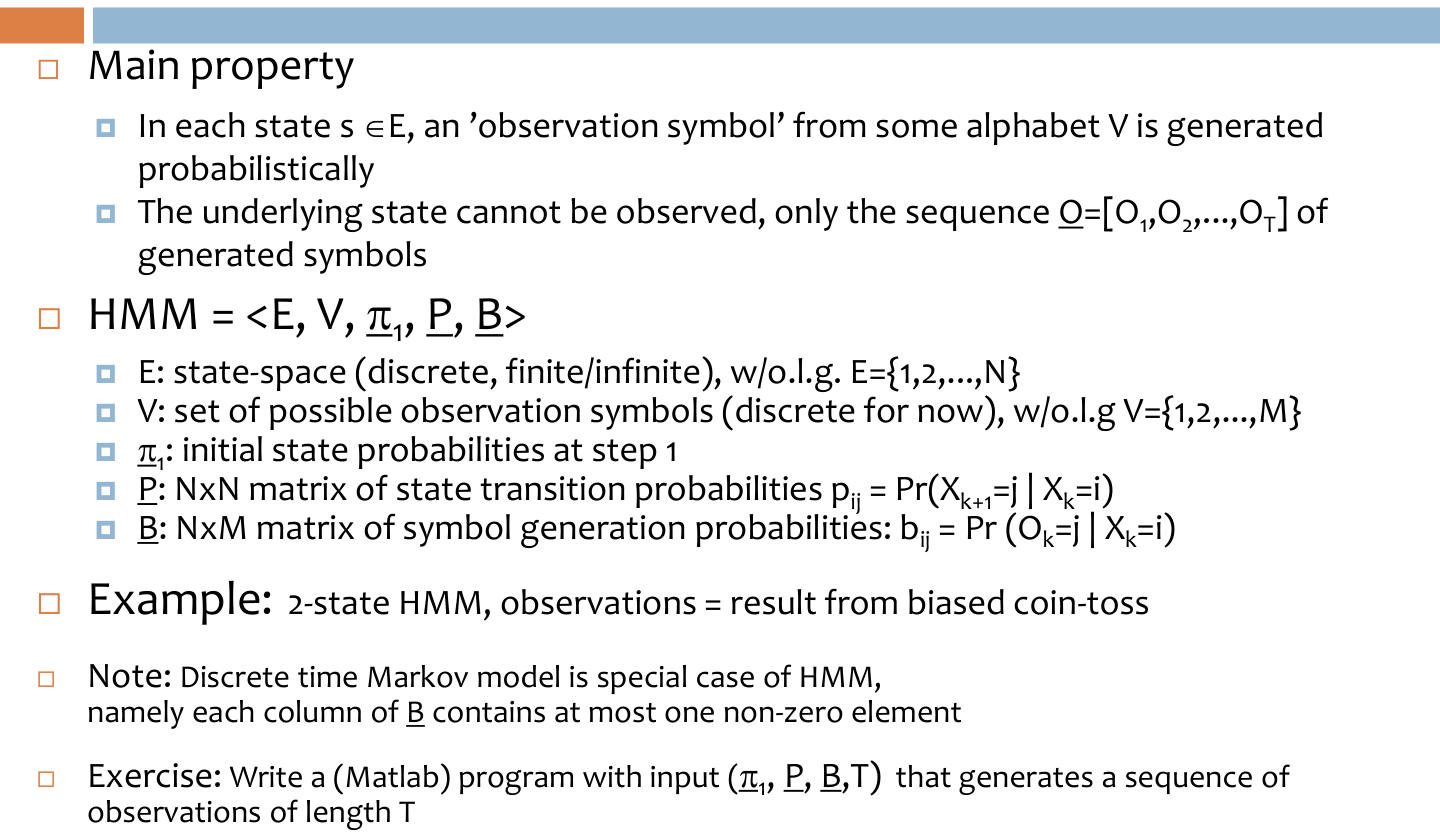
\includegraphics[width=\textwidth]{fig_hmm_definition.png}
  \caption{Formal definition of the HMM tuple and the generative model.
    At each time step the hidden state $X_k$ first transitions to $X_{k+1}$
    according to $\mathbf{P}$, and then emits an observable symbol $O_k$
    according to the row of $\mathbf{B}$ corresponding to $X_k$.
    Only the sequence of emitted symbols $O_1, O_2, \ldots, O_T$ is visible
    to the observer; the state sequence $X_1, X_2, \ldots$ is never seen
    directly.}
\end{figure}

An HMM is fully described by five components, written as the tuple
$\mathcal{M} = \langle E,\, V,\, \boldsymbol{\pi}_1,\, \mathbf{P},\,
\mathbf{B} \rangle$:

\begin{defbox}
  \textbf{HMM components --- what each element means:}
  \begin{itemize}[leftmargin=1.2em, itemsep=5pt]
    \item $E = \{1,\ldots,N\}$ --- the \textbf{state space}: the finite set of
      hidden states. In the wireless example $N=3$ (good, intermediate, poor).
    \item $V = \{1,\ldots,M\}$ --- the \textbf{observation alphabet}: the
      finite set of symbols that can be emitted. In the wireless example
      $M=2$ (C=correct, E=error).
    \item $\boldsymbol{\pi}_1$ --- the \textbf{initial state distribution}: a
      probability vector of length $N$; entry $i$ gives the probability of
      starting in state $i$ at step 1.
    \item $\mathbf{P}$ --- the $N \times N$ \textbf{state transition matrix}:
      entry $p_{ij} = \Pr(X_{k+1}=j \mid X_k=i)$ is the probability of
      transitioning from state $i$ to state $j$ in one time step. Each row
      sums to 1.
    \item $\mathbf{B}$ --- the $N \times M$ \textbf{emission matrix}: entry
      $b_{ij} = \Pr(O_k=j \mid X_k=i)$ is the probability of emitting symbol
      $j$ when in hidden state $i$. Each row sums to 1.
  \end{itemize}
\end{defbox}

\begin{notebox}
  \textbf{HMM versus plain Markov chain.}
  A plain DTMC is a special case of an HMM where each state emits exactly
  one unique symbol (each column of $\mathbf{B}$ has at most one non-zero
  entry). In that case the state is revealed directly by the emission, so
  nothing is hidden. The moment a state can emit \emph{multiple different
  symbols with non-zero probability}, or multiple states can emit the
  \emph{same} symbol, the state becomes hidden and we need the HMM framework.
\end{notebox}

% ==============================================================================
\section*{Part 5 \quad Efficient Algorithms for HMMs}
% ==============================================================================

Three fundamental computational problems arise when working with HMMs.
All three take the model $\mathcal{M} = \langle E, V, \boldsymbol{\pi}_1,
\mathbf{P}, \mathbf{B} \rangle$ and an observation sequence $\mathbf{o} =
[o_1, \ldots, o_T]$ as input, but ask different questions about them.
Problems 1 and 2 are the focus of this lecture.

% ------------------------------------------------------------------------------
\subsection*{5.1 \quad Problem 1: Observation Probability (Forward Algorithm)}
% ------------------------------------------------------------------------------

\textbf{Goal:} Given model $\mathcal{M}$ and observation sequence $\mathbf{o}$,
compute the total probability $\Pr(\mathbf{O} = \mathbf{o} \mid \mathcal{M})$
--- i.e.\ how likely is it that this particular HMM would produce this
particular sequence of observations?

This question arises in fault detection when we have \emph{two} trained HMMs
--- one for normal operation and one for faulty operation --- and want to decide
which is more consistent with what we currently observe.

A brute-force approach would enumerate every possible hidden state sequence
$\mathbf{q} = [q_1, \ldots, q_T]$, compute $\Pr(\mathbf{o} \mid \mathbf{q})$
for each, and sum. But there are $N^T$ possible sequences, which grows
exponentially. For $N=3$ states and $T=100$ observations that is
$3^{100} \approx 5 \times 10^{47}$ terms --- completely intractable.

The \textbf{forward procedure} solves the same problem in $O(N^2 T)$ time
(quadratic in states, linear in time) by building the answer incrementally,
one time step at a time.

\vspace{4pt}
\textbf{The forward variable} $\boldsymbol{\alpha}_t(i)$ captures everything
we need from the past up to step $t$:
\[
  \boldsymbol{\alpha}_t(i) := \Pr(O_1=o_1,\, O_2=o_2,\, \ldots,\, O_t=o_t,\; X_t=i).
\]
\begin{itemize}[leftmargin=1.4em, itemsep=2pt]
  \item $\boldsymbol{\alpha}_t(i)$ --- the joint probability that the first $t$
    observations match $o_1,\ldots,o_t$ \emph{and} the hidden state at time
    $t$ is $i$.
  \item $O_1, \ldots, O_t$ --- the random variables representing observations
    at steps 1 through $t$.
  \item $o_1, \ldots, o_t$ --- the specific observed values (symbols from $V$).
  \item $X_t$ --- the hidden state random variable at step $t$.
  \item $i$ --- a specific state from $E$.
\end{itemize}

\textbf{Algorithm:}
\begin{enumerate}[leftmargin=1.6em, itemsep=6pt]
  \item \textbf{Initialise} ($t=1$):
    \[
      \boldsymbol{\alpha}_1(i) = \pi_1(i)\,b_{i,\,o_1}
      \qquad \text{(Matlab: } \boldsymbol{\alpha}_1 = \boldsymbol{\pi}_1
      \mathbin{.*} \mathbf{B}(:,\,o_1)' \text{)}
    \]
    \begin{itemize}[leftmargin=1.2em, itemsep=2pt]
      \item $\pi_1(i)$ --- prior probability of starting in state $i$.
      \item $b_{i,\,o_1}$ --- probability of emitting the first observation $o_1$
        from state $i$ (row $i$, column $o_1$ of $\mathbf{B}$).
    \end{itemize}

  \item \textbf{Recurse} ($t = 1, \ldots, T-1$):
    \[
      \boldsymbol{\alpha}_{t+1}(j) =
      \left(\sum_{i \in E} \boldsymbol{\alpha}_t(i)\,p_{ij}\right)
      \cdot b_{j,\,o_{t+1}}
      \qquad \text{(Matlab: } \boldsymbol{\alpha}_{t+1} =
      (\boldsymbol{\alpha}_t\,\mathbf{P}) \mathbin{.*} \mathbf{B}(:,\,o_{t+1})' \text{)}
    \]
    \begin{itemize}[leftmargin=1.2em, itemsep=2pt]
      \item $\sum_{i \in E} \boldsymbol{\alpha}_t(i)\,p_{ij}$ --- sum over all
        states $i$ at step $t$, weighted by the transition probability $p_{ij}$
        to the next state $j$. This propagates all previous mass to state $j$.
      \item $b_{j,\,o_{t+1}}$ --- probability of emitting the next observation
        $o_{t+1}$ from state $j$. This gates the propagated mass by how
        consistent state $j$ is with what was just observed.
    \end{itemize}

  \item \textbf{Terminate}:
    \[
      \Pr(\mathbf{O}=\mathbf{o}) = \sum_{j \in E} \boldsymbol{\alpha}_T(j).
    \]
    \begin{itemize}[leftmargin=1.2em, itemsep=2pt]
      \item Sum the forward variable over all states at the final step $T$.
        This marginalises out the unknown final state, giving the total
        observation probability.
    \end{itemize}
\end{enumerate}

\begin{figure}[H]
  \centering
  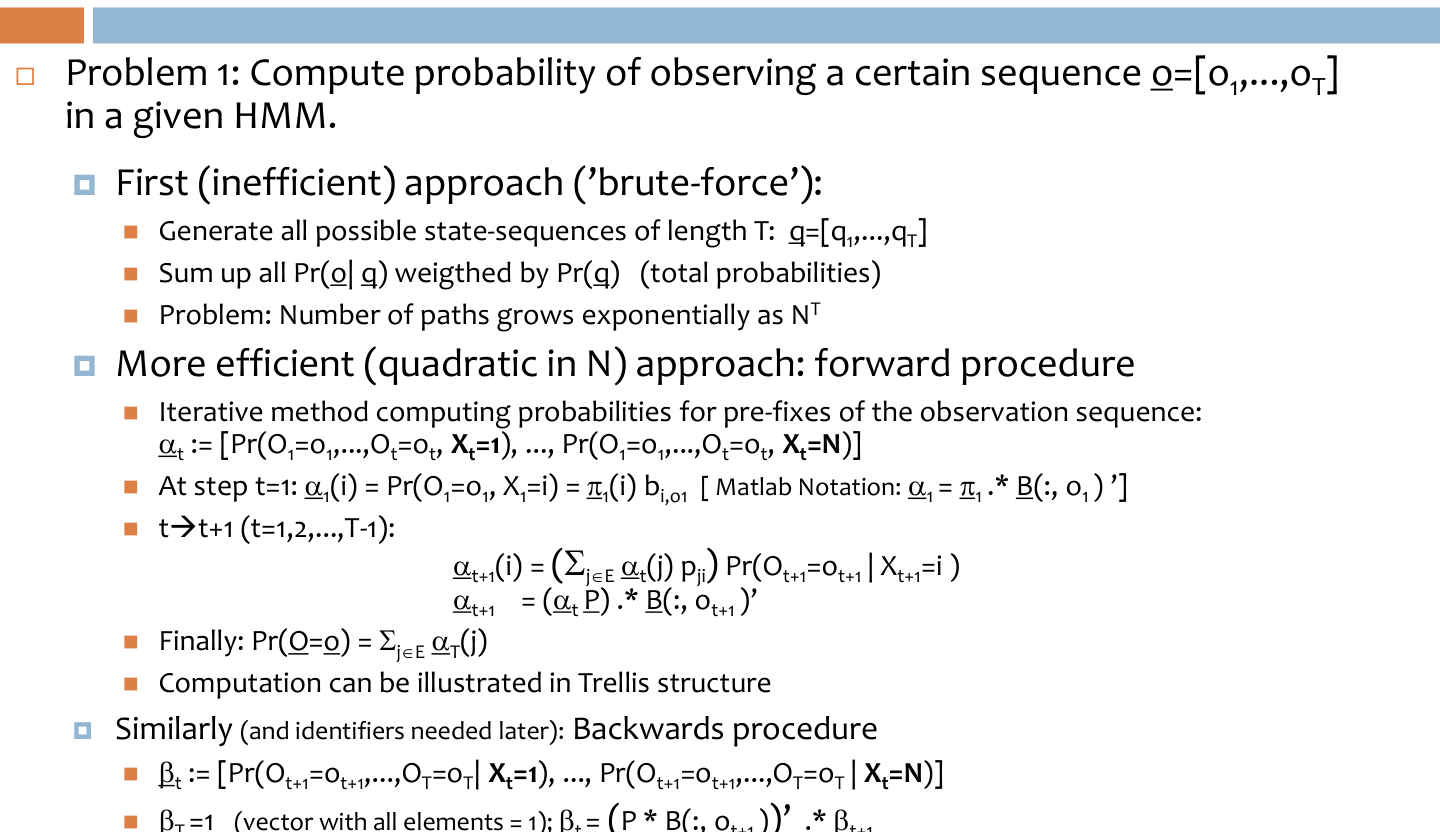
\includegraphics[width=\textwidth]{fig_forward_algorithm.png}
  \caption{The Forward Algorithm as presented in the slides, including the
    companion \textbf{backward procedure}.
    The backward variable $\boldsymbol{\beta}_t(i) = \Pr(O_{t+1}=o_{t+1},
    \ldots, O_T=o_T \mid X_t=i)$ captures the probability of all
    \emph{future} observations given that the hidden state at $t$ is $i$.
    It is initialised as an all-ones vector at $T$ and propagated backwards
    to $t=1$. The backward variable is not needed for Problems~1 or~2 but
    is required for the Baum-Welch fitting algorithm (Problem~3).}
\end{figure}

\begin{notebox}
  \textbf{Why dynamic programming works here.}
  The forward variable $\boldsymbol{\alpha}_t$ is a vector of length $N$ that
  compresses the entire history into just $N$ numbers. At each step we need
  only $N^2$ multiplications to update it (one per $(i,j)$ pair in $\mathbf{P}$).
  Contrast this with the brute-force approach which would need to keep track
  of all $N^t$ path prefixes explicitly. Dynamic programming discards the
  path details while retaining the probabilities --- the same principle as the
  Chapman-Kolmogorov recursion for Markov chains.
\end{notebox}

% ------------------------------------------------------------------------------
\subsection*{5.2 \quad Problem 2: Most Likely State Sequence (Viterbi Algorithm)}
% ------------------------------------------------------------------------------

\textbf{Goal:} Given model $\mathcal{M}$ and observation sequence $\mathbf{o}$,
find the specific hidden-state sequence $\mathbf{q}^* = [q_1^*, \ldots, q_T^*]$
that is most likely to have generated those observations. Formally, find:
\[
  \mathbf{q}^* = \arg\max_{\mathbf{q}} \;\Pr(X_1=q_1, \ldots, X_T=q_T
  \mid \mathbf{O}=\mathbf{o}).
\]
\begin{itemize}[leftmargin=1.4em, itemsep=2pt]
  \item $\mathbf{q}^*$ --- the optimal (most likely) hidden state sequence.
  \item $\arg\max_{\mathbf{q}}$ --- the argument that maximises the expression;
    i.e.\ the state sequence $\mathbf{q}$ achieving the highest probability.
  \item The conditional is over all $N^T$ possible sequences $\mathbf{q}$,
    but the Viterbi algorithm finds the maximum without enumerating them all.
\end{itemize}

For fault detection this is the key question: given what I have observed so
far, what is the most likely sequence of system states? If the answer ends in
a fault state, we declare a fault.

The structure is identical to the Forward Algorithm but with $\max$ replacing
$\sum$. However, because we need to reconstruct the best path (not just its
probability), we must also store a \textbf{backpointer} at every step.

\vspace{4pt}
\textbf{The Viterbi variable} $\boldsymbol{\delta}_t(i)$ is the probability
of the single best path ending in state $i$ at time $t$:
\[
  \boldsymbol{\delta}_t(i) :=
  \max_{q_1, \ldots, q_{t-1}}
  \Pr\!\left(X_1=q_1,\ldots,X_{t-1}=q_{t-1},\, X_t=i,\;
      O_1=o_1,\ldots,O_t=o_t\right).
\]
\begin{itemize}[leftmargin=1.4em, itemsep=2pt]
  \item $\boldsymbol{\delta}_t(i)$ --- the joint probability of the best
    partial path up to step $t$ that ends in state $i$, together with
    all observations $o_1, \ldots, o_t$.
  \item The $\max$ is over all possible ways to get to state $i$ at time $t$
    via any sequence of earlier states.
\end{itemize}

The \textbf{backpointer} $\Psi_{t+1}(j)$ records which previous state was
optimal:
\[
  \Psi_{t+1}(j) = \arg\max_{i=1,\ldots,N} \boldsymbol{\delta}_t(i)\,p_{ij}.
\]
\begin{itemize}[leftmargin=1.4em, itemsep=2pt]
  \item $\Psi_{t+1}(j)$ --- the state at step $t$ that maximises the path
    probability when followed by state $j$ at step $t+1$. Stored for every
    $(t+1, j)$ pair so the best path can be traced backwards at the end.
  \item $p_{ij}$ --- transition probability from state $i$ to $j$.
\end{itemize}

\begin{figure}[H]
  \centering
  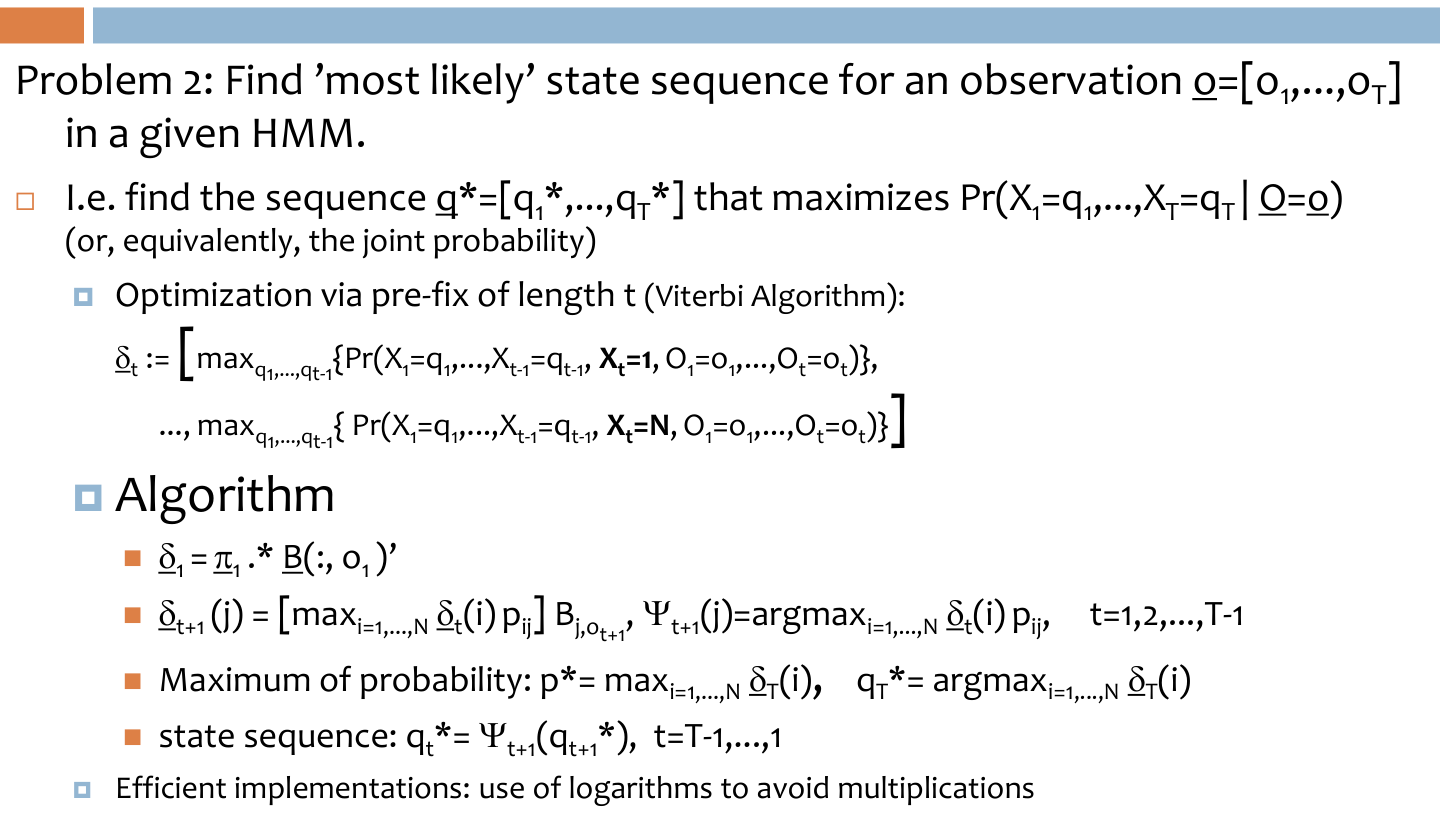
\includegraphics[width=\textwidth]{fig_viterbi_algorithm.png}
  \caption{The Viterbi Algorithm as shown in the slides.
    The algorithm fills a $N \times T$ grid (the \emph{trellis}) where each
    cell holds $\boldsymbol{\delta}_t(i)$. At each column only the single
    best predecessor is kept (via $\Psi$), discarding all sub-optimal
    partial paths. After filling the grid, the optimal last state is found
    from column $T$, and the full path is recovered by following the
    backpointers leftward.}
\end{figure}

\textbf{Full algorithm:}
\begin{enumerate}[leftmargin=1.6em, itemsep=6pt]
  \item \textbf{Initialise} ($t=1$):
    \[
      \boldsymbol{\delta}_1 = \boldsymbol{\pi}_1 \mathbin{.*} \mathbf{B}(:,\,o_1)'
    \]
    Same as the Forward initialisation --- the best path of length 1 ending in
    state $i$ has probability $\pi_1(i)\,b_{i,o_1}$.

  \item \textbf{Recurse} ($t = 1, \ldots, T-1$):
    \[
      \boldsymbol{\delta}_{t+1}(j) =
      \left[\max_{i=1}^{N} \boldsymbol{\delta}_t(i)\,p_{ij}\right]
      \cdot B_{j,\,o_{t+1}},
      \qquad
      \Psi_{t+1}(j) = \arg\max_{i=1}^{N} \boldsymbol{\delta}_t(i)\,p_{ij}.
    \]
    \begin{itemize}[leftmargin=1.2em, itemsep=2pt]
      \item $\max_{i} \boldsymbol{\delta}_t(i)\,p_{ij}$ --- among all states
        $i$ at step $t$, pick the one that gives the highest path probability
        when transitioning to state $j$.
      \item $B_{j,\,o_{t+1}}$ --- gate by emission probability, just like the
        Forward recursion.
      \item $\Psi_{t+1}(j)$ --- records which $i$ achieved that maximum, so
        we can later reconstruct the path.
    \end{itemize}

  \item \textbf{Terminate}:
    \[
      p^* = \max_{i=1}^{N} \boldsymbol{\delta}_T(i), \qquad
      q_T^* = \arg\max_{i=1}^{N} \boldsymbol{\delta}_T(i).
    \]
    \begin{itemize}[leftmargin=1.2em, itemsep=2pt]
      \item $p^*$ --- probability of the overall best path.
      \item $q_T^*$ --- the optimal final state (at time $T$).
    \end{itemize}

  \item \textbf{Backtrack} ($t = T-1, \ldots, 1$):
    \[
      q_t^* = \Psi_{t+1}(q_{t+1}^*).
    \]
    Follow the stored backpointers from the end of the sequence back to the
    start to recover the full state path $[q_1^*, \ldots, q_T^*]$.
\end{enumerate}

\begin{keybox}
  \textbf{Viterbi vs.\ Forward --- same structure, different question.}
  Both algorithms run in $O(N^2 T)$ and initialise identically.
  \begin{itemize}[leftmargin=1.2em, itemsep=2pt]
    \item \textbf{Forward} uses $\boldsymbol{\alpha}_{t+1} = (\boldsymbol{\alpha}_t \mathbf{P})
      \mathbin{.*} \mathbf{B}(\cdot, o_{t+1})$, summing over predecessor states
      --- answers ``how probable is this observation sequence?''
    \item \textbf{Viterbi} replaces $\sum$ with $\max$ and stores
      $\Psi$ --- answers ``what state sequence most likely produced it?''
  \end{itemize}
  In practice both algorithms use logarithms throughout to turn products of
  small probabilities into sums of log-probabilities, avoiding numerical
  underflow.
\end{keybox}

% ------------------------------------------------------------------------------
\subsection*{5.3 \quad Problem 3: HMM Parameter Fitting (Baum-Welch)}
% ------------------------------------------------------------------------------

\textbf{Goal:} Given an observation sequence $\mathbf{o}$ and assumed state
space $E$ and observation alphabet $V$, find the model parameters
$\langle \boldsymbol{\pi}_1^*, \mathbf{P}^*, \mathbf{B}^* \rangle$ that
maximise $\Pr_{\mathcal{M}}(\mathbf{O}=\mathbf{o})$:
\[
  \langle \boldsymbol{\pi}_1^*, \mathbf{P}^*, \mathbf{B}^* \rangle
  = \arg\max_{\boldsymbol{\pi}_1,\,\mathbf{P},\,\mathbf{B}}\;
  \Pr_{\langle \boldsymbol{\pi}_1,\,\mathbf{P},\,\mathbf{B} \rangle}
  (\mathbf{O} = \mathbf{o}).
\]
\begin{itemize}[leftmargin=1.4em, itemsep=2pt]
  \item $\boldsymbol{\pi}_1^*, \mathbf{P}^*, \mathbf{B}^*$ --- the optimal
    initial distribution, transition matrix, and emission matrix respectively,
    chosen to make the observed data as probable as possible under the model.
  \item $\Pr_{\mathcal{M}}(\cdot)$ --- probability computed with a specific
    model $\mathcal{M}$; the subscript makes clear that the probability
    depends on the model parameters being optimised.
\end{itemize}

This is solved by the \textbf{Baum-Welch} algorithm (a special case of the
EM algorithm). It iteratively re-estimates all parameters using the forward
and backward variables, and is guaranteed to increase the observation
likelihood at each iteration (or leave it unchanged at convergence).
Convergence to a \emph{local} maximum is the main risk, so multiple random
initialisations are used in practice. This algorithm is \emph{not} examinable
in this lecture but forms the basis for training HMM-based detectors on
real measurement data.

% ==============================================================================
\section*{Part 6 \quad HMM-Based Fault Detection}
% ==============================================================================

% ------------------------------------------------------------------------------
\subsection*{6.1 \quad Single Observation: Congestion Detector}
% ------------------------------------------------------------------------------

Now we put everything together and use an HMM as a fault detector.
The congestion example from Part~2 used a simple threshold on a single RTT
measurement. The HMM-based approach is more powerful because it considers a
\emph{sequence} of RTT measurements and takes into account that congestion
states tend to persist over time (captured by the Markov transition structure).

\begin{figure}[H]
  \centering
  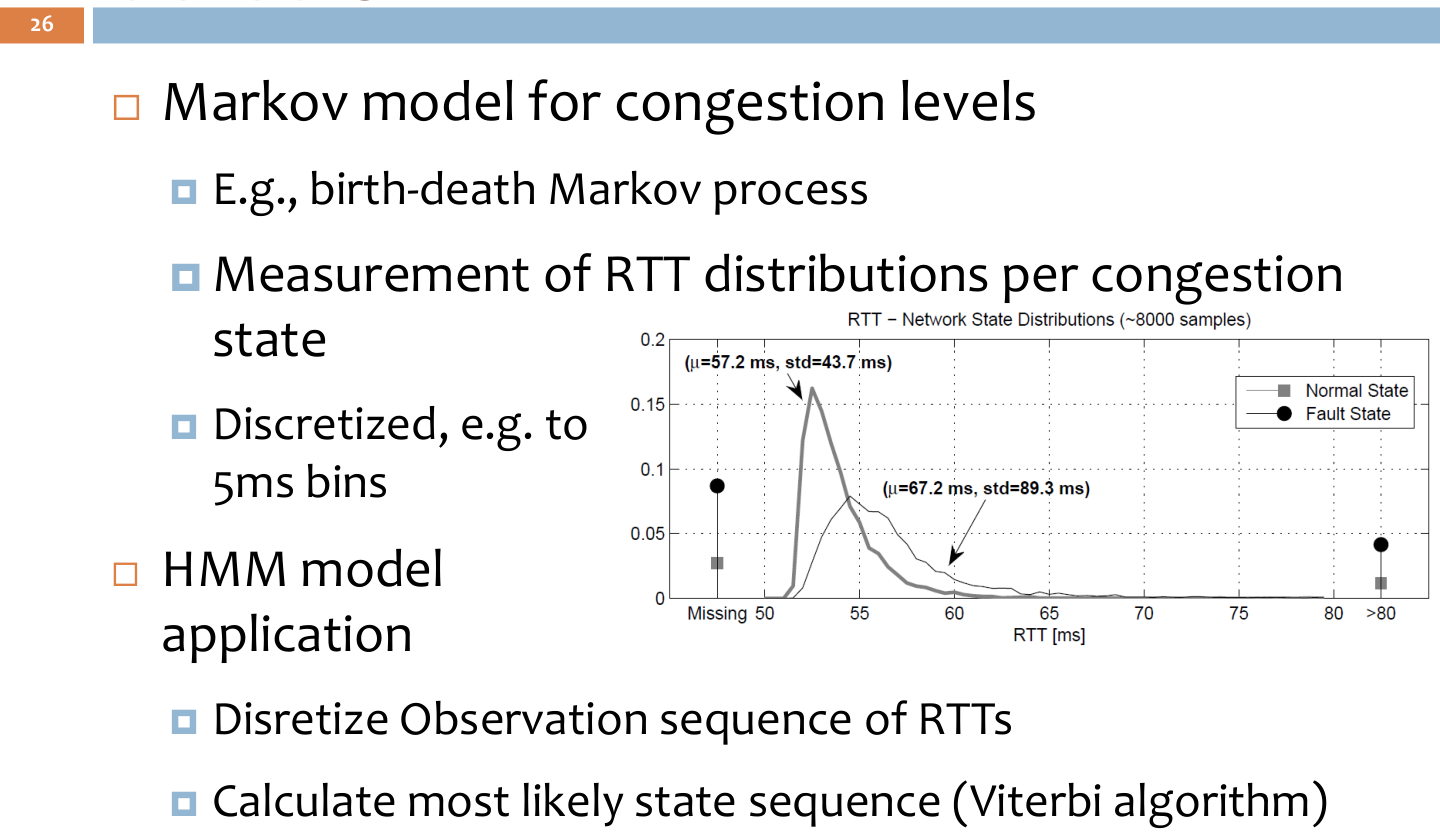
\includegraphics[width=0.85\textwidth]{fig_hmm_congestion.png}
  \caption{Mapping the congestion detection problem onto an HMM.
    \textbf{Left}: the hidden states are congestion levels (e.g.\ a
    birth-death Markov chain where congestion can only increase or decrease by
    one level per step).
    \textbf{Right}: the RTT distribution is measured separately for each
    congestion state and discretised into bins (e.g.\ 5\,ms bins) to form the
    rows of the emission matrix $\mathbf{B}$.
    At runtime, a stream of observed RTT values is fed to the Viterbi
    algorithm, which outputs the most likely congestion state at each step.
    A fault is declared whenever that state exceeds a chosen severity level.}
\end{figure}

The key steps to build and apply an HMM-based fault detector:
\begin{enumerate}[leftmargin=1.6em, itemsep=4pt]
  \item \textbf{Model the system state} as a Markov chain. Choose states that
    correspond to meaningful operating conditions (healthy, mildly degraded,
    severely congested, \ldots). Estimate the transition matrix $\mathbf{P}$
    from historical fault-occurrence data.
  \item \textbf{Characterise emissions}: for each state, measure the
    distribution of the observable (here RTT). Discretise it into $M$ bins to
    form one row of $\mathbf{B}$.
  \item \textbf{Collect a sequence of observations} at runtime. A single
    sample gives little information; a sequence of samples allows the HMM to
    exploit temporal patterns.
  \item \textbf{Apply the Viterbi algorithm} to the observation sequence to
    recover the most likely hidden-state sequence.
  \item \textbf{Declare a fault} whenever the most likely current state is a
    fault state.
\end{enumerate}

\begin{notebox}
  \textbf{Why sequences are more informative than single samples.}
  A single RTT spike could be a random packet delay in a perfectly healthy
  network, or it could be the beginning of congestion.
  The HMM distinguishes between these because the Markov transition structure
  assigns a higher probability to a state \emph{persisting} than to a state
  appearing and disappearing within one step.
  A sustained pattern of high RTTs is therefore much stronger evidence of
  congestion than a single high RTT.
\end{notebox}

% ------------------------------------------------------------------------------
\subsection*{6.2 \quad Multiple Faults and Observations}
% ------------------------------------------------------------------------------

A major strength of the HMM framework is that it generalises naturally to
scenarios with \emph{multiple simultaneous fault types} and \emph{multiple
observable signals}.

\begin{figure}[H]
  \centering
  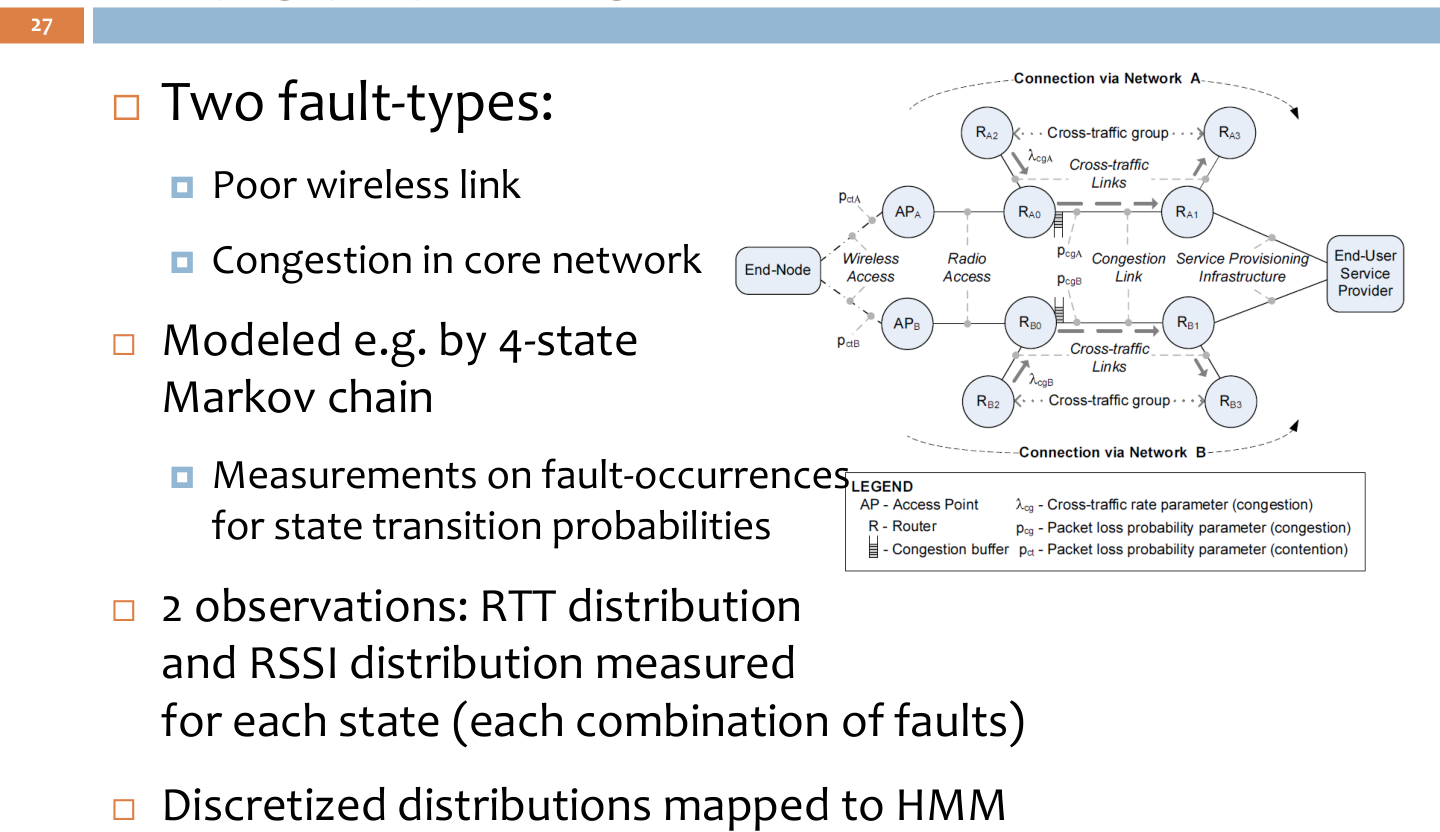
\includegraphics[width=\textwidth]{fig_multi_fault.png}
  \caption{Network topology with two possible fault types occurring
    independently: \textbf{poor wireless link} (between the end-node and the
    access point) and \textbf{congestion in the core network} (in the routers
    between the access point and the service provider).
    Because these faults are independent, they can combine into four distinct
    system states: (no fault, no fault), (wireless fault only), (congestion
    only), and (both faults).
    Two observations are available: \textbf{RTT} (sensitive to congestion)
    and \textbf{RSSI} (Received Signal Strength Indicator, sensitive to
    wireless link quality).
    The joint emission matrix $\mathbf{B}$ contains the discretised RTT and
    RSSI distributions for each of the four states, giving the HMM all the
    information it needs to diagnose which fault (if any) is active.}
\end{figure}

The two observations (RTT and RSSI) serve complementary roles:
\begin{itemize}[leftmargin=1.4em, itemsep=3pt]
  \item \textbf{RTT} is large when there is congestion in the core network
    (packets queue in routers), but is unaffected by wireless signal strength.
  \item \textbf{RSSI} (Received Signal Strength Indicator) measures the power
    of the received radio signal. A low RSSI indicates poor wireless link
    conditions and correlates with high frame error rates, but RSSI is
    unaffected by core-network congestion.
\end{itemize}
By combining both signals in one HMM, the algorithm can distinguish all four
system states --- something that neither signal alone can do reliably.

\begin{notebox}
  \textbf{Advantages of HMM-based detectors over threshold detectors.}
  \begin{itemize}[leftmargin=1.2em, itemsep=3pt]
    \item \textbf{Temporal correlations}: a sustained sequence of high RTTs is
      far more convincing evidence of congestion than a single spike.
    \item \textbf{Multiple simultaneous faults}: handled by adding states to
      the Markov chain (one state per combination of active faults).
    \item \textbf{Multiple observations}: different signals inform different
      parts of $\mathbf{B}$, giving cross-layer diagnostic power.
    \item \textbf{Learnable}: if the distributions are unknown, Baum-Welch
      can estimate $\mathbf{P}$ and $\mathbf{B}$ directly from data.
  \end{itemize}
\end{notebox}

% ==============================================================================
\section*{Part 7 \quad Key Points Summary}
% ==============================================================================

\begin{keybox}
  \textbf{Discrete-Time Markov Model elements:}
  a finite state space $E$; a transition probability matrix $\mathbf{P}$
  (row $j$ gives the distribution over next states from state $j$); an
  initial distribution $\boldsymbol{\pi}_0$.
\end{keybox}

\begin{keybox}
  \textbf{HMM elements:}
  an underlying DTMC $(\boldsymbol{\pi}_1, \mathbf{P})$ describing how the
  \emph{hidden} state evolves, plus an emission matrix $\mathbf{B}$ linking
  each hidden state to a probability distribution over an observable alphabet
  $V$. The observer sees only the emitted symbols, never the states directly.
\end{keybox}

\begin{keybox}
  \textbf{Three HMM problems and their algorithms:}
  \begin{enumerate}[leftmargin=1.4em, itemsep=3pt]
    \item \textbf{Observation probability} --- how likely is this observation
      sequence under this model? Solved by the \textbf{Forward algorithm}
      in $O(N^2 T)$.
    \item \textbf{Most likely state sequence} --- what hidden states most
      plausibly produced these observations? Solved by the \textbf{Viterbi
      algorithm} in $O(N^2 T)$.
    \item \textbf{Parameter fitting} --- given data, find the best $\mathbf{P}$
      and $\mathbf{B}$. Solved by \textbf{Baum-Welch (EM)}; converges to a
      local optimum.
  \end{enumerate}
\end{keybox}

% ==============================================================================
\section*{References}
% ==============================================================================

\begin{itemize}[leftmargin=1.4em, itemsep=4pt]
  \item L.~Rabiner, ``A Tutorial on Hidden Markov Models and Selected
    Applications in Speech Recognition,'' \emph{Proc.\ IEEE}, vol.~77,
    no.~2, Feb.\ 1989.
  \item J.~Grønbæk, \emph{Decentralized Fault Management for Service
    Dependability in Ubiquitous Networks}, PhD Thesis, Aalborg University,
    Oct.\ 2010.
  \item A.~Nickelsen, J.~Gronbak, T.~Renier, and H.-P.~Schwefel,
    ``Probabilistic Fault-Diagnosis in Mobile Networks Using Cross-Layer
    Observations,'' in \emph{Proc.\ AINA 2009}, Bradford, UK, May 2009.
  \item A.~Bondavalli et al., ``Threshold-based mechanisms to discriminate
    transient from intermittent faults,'' \emph{IEEE Trans.\ Comput.},
    49(3):230--245, 2000.
\end{itemize}

\end{document}
